\documentclass[12pt]{article}
\usepackage{graphicx}
\begin{document}
\begin{center}
\textbf{CHAPTER-7}\\
\vspace{2\bigskipamount}
\textbf\textbf\large{Straight Line and Pair of Straight Lines}


\end{center}
\section*{Section-A    JEE Advanced/IIT-JEE}
\section*{A      Fill in the Blanks}

1. The area enclosed within the curves $|x|+|y|$ is.........\\
2. $y=10^x$ is the reflection of $y=\log_10^x $ in the line whose equation is.........\\
3. The set of lines $ax+by+c=0$ where $3a+2b+4c=0$ is concurrent at the point..........\\
4. Given the points A(0,4) and B(0,-4), the equation of the locus of the point P(x,y) such that$|AP-BP|=6$ is.............\\
5. If $a,b and c$ are in A.P..then the straight line $ax+by+c=0$ will always pass through a fixed point whose coordinates are.........\\
6. The orthocenter of the triangle formed by the lines $x+y=1, 2x+3y=6  and  4x-y+4=0$ lies in quadrant number............\\
7. Let the algebraic sum of the perpendicular distances from the points (2,0), (0,2) and (1,1)to a variable straight line be zero; then the line passes through a fixed point whose cordinates are.........\\
8. The vertices of a triangle are  A(-1,-7), B(5,1)and C(1,4). The equation of the bisector of the angle $\angle{ABC}$ is............\\

\section*{B         True/False}

1. The sraight line $5x+4y=0$ passes through the point of intersection of the straight lines $x+2y-10=0$ and $2x+5+6=0$.\\
2. The lines $2x+3y=19=0$ $9x+6y-17=0$ cut the coordinate axes in concyclic points.\\

\section*{C   MCQ'S with One Correct Answer}

1. 	The points$(a,b),(0,0)(a,b)$ and $(a2.ab)$ are:\\
a .Clinear\\
b.Vrtices of a parallelogram\\
c. Vertices of a rectangle\\
d. None of the above\\
2. The point $(4,1)$ undergose thev  following three transformations successivvely.\\
i.Reflection about the line y=x\\
 ii.Translation through a distance 2 unit along the positivedirection of x-axis.\\
iii. Rotation through an angle p/4 about the origin the counter clockwise direction.\\
then the final position of the point is given by the coordinates.\\
(a)     $\frac{1}{\sqrt{2}},\frac{7}{\sqrt{2}}$   \hspace{1cm}  (b)     $(-\sqrt{2}, \sqrt[7]{2})$  \hspace{1cm} (c)    $\frac{-1}{\sqrt{2}},\frac{7}{\sqrt{2}}$ \hspace{1cm}(d)     $(\sqrt{2}, \sqrt[7]{2})$\\
3. The straight lines $x+y=0, 3x+y-4=0,x+3y-4=0$ from a triangle which is \\
(a) isoscales \hspace{1cm}   (b) equilateral  \hspace{1cm}  (c)  right angled  \hspace{1cm}  (d)  none of these \\
4. If $P=(1,0), Q=(-1,0) and R=(2,0)$ are three given
points, then  the locus  of the point S satisfying the relaion $SQ^2+SR^2=SP^2$, is\\
(a)  a straight line parllel to x-axis  \hspace{1cm}   (b) a circie passing hrough the origin \hspace{1cm}(c)  a circle with the center at the origin  \hspace{1cm}  (d)  a straight line parllel to y-axis\\
5. Line L has intercepts a and b on the coordinate axes. Wen the axes are rotatwd through a given ange,keeingup the origin fixed,the same ine L has intercepts  pand q then\\
(a)  $a^2=b^2=p^2=q^2$ \hspace{1cm}(b)  $\frac{1}{a^2} +\frac{1}{b^2}= \frac{1}{p^2}=\frac{1}{q^2}$ \hspace{1cm}  (c) $a^2+p^2=b^2+q^2$ \hspace{1cm}(d) $\frac{1}{a^2}+\frac{1}{p^2}=\frac{1}{b^2}+\frac{1}{q^2}$\\
6. If the sum of the distance of point from two perpendicular lines in a plane is 1,then its locu's is \\
(a) square \hspace{1cm}  (b) circle \hspace{1cm} (c)  straight line  \hspace{1cm}(d)  two intersecting lines\\
7. The locus of the vaiable point whose distance from from $(-2,0)$ is 2/3 times it's distance from the line $x=\frac{-9}{2}$ is\\
(a) elipse  \hspace{1cm} (b)  parabola  \hspace{1cm} (c) hyperbola   \hspace{1cm}  (d) none of the above\\
8. The equation to a pair of  opposite sides of parallelogram are $x^2-5x+6=0$ and $y^2-6y+5=0$ the equations to it's diagonals are\\
(a)  $x+4y=13, y=4x-7$  \hspace{1cm} (b)   $4x+y=13, 4y=x-7$ \hspace{1cm}   (c)  $4x+y=13, y=4x-7$\\
(d)  $y-4x=13,y+4x=7$ \\
9. The orthocenter of the lines formed by $xy=0$ and $x+y=1$ is\\
(a)  (1/2,1/2) \hspace{1cm} (b)  (1/3,1/3) \hspace{1cm}  (c)  (0,0) \hspace{1cm} (d)  (1/4,1/4)\\
10. Let PQR be a rightangled isoscales triangle, right angled at $P(2,1)$ if the equation of the line QR is $2x+y=3$, then the equation representing the pair of line PQ and PR is\\
(a)  $3x^2-3y^2+8xy+20x+10y+25=0$\hspace{1cm} (b)  $3x^2-3y^2+8xy-20x-10y+25=0$\\
(c)  $3x^2-3y^2+8xy+10x+15y+20=0$\hspace{1cm}(d)  $3x^2-3y^2-8xy-10x-15y-20=0$\\
11. If $x_1,x_2,x_3$ as well as $y_1,y_2,y_3 $are in GP with the same common ratio, then the points $(x_1,y_1),(x_2,y_2)$ and $(x_3,y_3)$\\
(a)  lie on a straight line \hspace{1cm}  (b)   lie on a elipse \hspace{1cm}  (c)  lie on a circle  \hspace{1cm} (d)   are vertices of trianngle \\
12. Let PS median of the tringle with vertices P(2,2), Q(6,1) and R(7,3). The equation of the line passing through (1,-1) and parllel to PS is.\\
(a)  $2x-9y-7=0$ \hspace{1cm}  (b)   $2x-9y-11=0$ \hspace{1cm}  (c)  $2x+9y-11=0$ \hspace{1cm} (d)  $2x+9y+7=0$\\
13. The incenter of the triangle with vertices $\frac{1}{\sqrt{3}}$,$(0,0)$ and $(2,0)$ is\\
(a) $[1,\sqrt{3}/2]$ \hspace{1cm} (b)  $\frac{2}{3}\,\frac{\sqrt{3}}{2}$ \hspace{1cm} (c)  $\frac{2}{3},\frac{\sqrt{3}}{2}$  \hspace{1cm} (d)  $[1,{1}{\sqrt{3}}]$\\
14. The number of integer values of m, for which the x-coordinate of the of intersection of line $3x+4y=9$ and $y=mx+1$ is also an integer, is\\
(a)  2  \hspace{1cm} (b)  0 \hspace{1cm} (c)  4   \hspace{1cm} (d)  1\\
15. Area of parllelogram formed by the lines $y=mx$, $y=mx+1$,  $y=nx$ and  $y=nx+1$ equals\\
(a) $\frac{\mid m+n\mid}{(m-n)^2}$\hspace{1cm}
(b) $\frac{2}{\mid m+n \mid}$\hspace{1cm}
(c) $\frac{1}{(\mid m+n \mid)}$\hspace{1cm}
(d) $\frac{1}{(\mid m-n\mid)}$\\
16. Let $0<a<\frac{\pi}{2}$ be fixed ange. If $P=(\cos\theta,\sin\theta)$, Q=$(\cos\alpha-\theta),(\sin\alpha-\theta)$, then Qis obtained from P by\\
(a)  clockwise wise rotation around origin through an angle $\alpha$\\
(b) anticlockwise wise rotation around origin through an angle $\alpha$\\
(c) reflection in the line through origin with slope $\tan\alpha$\\
(d) reflection in the line through origin with slope $\tan\alpha/2$\\
17. Let $P=(-1,0)$,$Q=(0,0)$ and $R=(3,\sqrt[3]{3})$ be three points.\\
Then the equation of the bisector of the angle PQR is\\
(a)  $\frac{\sqrt{3}}{2x}+y=0$ \hspace{1cm}           (b)   $(x+\sqrt{3}y=0)$\\
(c)  $\sqrt{3}x+y=0$  \hspace{1cm}       (d)  $x+\frac{\sqrt{3}}{2y}=0$\\
18. A straight line through the origin O meets the parllel lines $4x+2y=9$ and $2x+y+6=0$ at points P and Q respectively. Then the point O divides the segment PQ in the ratio\\
(a) $1:2$   \hspace{1cm} (b) $3:4$  \hspace{1cm}  (c) $2:1$ \hspace{1cm}   (d) $4:3$ \\
19.The number of integral points(integral points means both the coordinates should be integer) exactly in the interior of the triangle with vertices is $(0,0)(0,21)$ and $(21,0)$ is\\
(a)  133   \hspace{1cm}  (b)  190  \hspace{1cm}   (c)  233 \hspace{1cm}  (d)   105\\
20. Orthocenter of triangle with vertices $(0,0)(3,4)$ and $(4,0)$ is \\
(a) $[3,\frac{5}{4}]$ \hspace{1cm} (b)$[3,12]$   \hspace{1cm} (c)  $[3,\frac{3}{4}]$   \hspace{1cm} (d)$[3,9]$\\
21. Aear of the triangr formed by the line $x+y=3$ and angle bisectors of the pair of straight ines $x^2-y^2+2y=1$\\
(a)  2 sq. units  \hspace{1cm}   (b)  4 sq. units  \hspace{1cm}    (c)  6 sq. units     \hspace{1cm} (d)  8 sq. units\\
22. Let $O(0,0),P(3,4),Q(6,0)$ be the vertices of the tiangles OPQ. The point R inside the triangle OPQ is such that the triangles OPR,PQR,,OQR are of equal area. The coordinates of R are \\
(a)  $[\frac{4}{3}, 3]$   \hspace{1cm}(b) $[3, \frac{2}{3}]$  \hspace{1cm}  (c)   $[3, \frac{4}{3}]$  \hspace{1cm}  (d)  $[\frac{4}{3}, \frac{2}{3}]$\\
23. A straight line through the point $(3,2)$ inclined at an angle $ 60^\circ $  to the line $\sqrt{3}x+y=1$. If L also intersects the x axis, then the equation of L is \\
(a) $y+\sqrt{3}+2+\sqrt[3]{3}=0$ \hspace{1cm} (b)   $y-\sqrt{3}+2+\sqrt[3]{3}=0$\\
(c)  $\sqrt{3}y-x+3+\sqrt[2]{3}=0$ \hspace{1cm} (d)   $\sqrt{3}y+x-3+\sqrt[2]{3}=0$\\

\section*{D -  MCQ'S with One or More Than One Correct Answer}

1. Three lines $px+qy+r=0$, $qx+ry+p=0$ and $rx+py+q=0$ are concurrent if \\
(a)  $p+q+r=0$\hspace{1cm} (b)  $p^2+q^2+r^2=qr+rp+pq$\hspace{1cm} (c)  $p^3+q^3+r^3=3pqr$\hspace{1cm} (d)  none of these\\
2. The points $[0,\frac{8}{3}]$,$[1,3]$ and $[82,30]$ are vertices of\\
(a)  an obtuse angle triangle\\
(b)  an acute angle triangle \\
(c)  a right angled triangle \\
(d)  an isoscales triangle\\
(e)  none of these\\
3. All points lying inside the triangle are formed by the points$(1,3)$,$(5,0)$ and $(-1,2)$ satisfy\\
(a)  $3x+2y\ge=0$\hspace{1cm} (b)  $2x+3y-13\ge=0$\hspace{1cm} (c)  $2x-3y-12\le=0$\hspace{1cm} (d)  $-2x+y\ge=0$\\
(e)  none of these\\
4.  A vector $\bar{a}$ has components of 2p and l with respect to a rectangular cartesian system. This system is rotted through a certain angle about origin in the counter clockwise sense. If,ith respect the new system,$\bar{a}$ has components $p+l$ and l, then\\
(a) $p=0$  \hspace{1cm}   (b)  $p=1$ or $p=-1/3$  \\
(c)  $p=-1$ or $p=1/3$  \hspace{1cm}(d)  $p=1$ or $p=-1$\\
(e) none of these.\\
5. If $P(1,2),Q(4,6),R(5,7)$ and $S(a,b)$ are the vertices of a parallelogram PQRS, then\\
(a)  $a=2,b=4$\hspace{1cm} (b)  $a=3,b=4$ \hspace{1cm}(c)  $a=2,b=3$\\
(d)  $a=3,b=5$\hspace{1cm} (e)  none of these\\
6. The diagonals of a parallelogram PQRS are along the lines $x+3y=4$ and $6x-2y=7$ then PQRS must be a.\\
(a) rectangle\\\hspace{1cm} (b) square\hspace{1cm} (c) cyclic quadrilateral\\
(d) rhombus\\
7. If the vertices P,Q,R of a triangle PQR are rational points, which of the following points of the triangle PQR is (are) always rational point(s)?\\
(a) centroid \hspace{1cm}   (b)  incenter\\
(c) circumcenter \hspace{1cm} (d) orthocenter\\
(A rational point is a point both of whose coordinates are rational numbers.)\\
8. Let $L_1$ be a straight line passing through the origin and $L_2$ be the straight line $x+y=1$. If the intercepts made by the circle $x^2+y^2-x+3y=0$ on $L_1$ and $L_2$ are equal, then which of the equation can represents $L_1$?\\
(a) $x+y=0$   \hspace{1cm} (b) $x-y=0$ \\ 
(c) $x+7y=0$   \hspace{1cm} (d) $x-7y=0$\\
9. For $a>b>c>0$, the distance between (1,1) and the point of intersection of the lines $ax+by+c=0$ and $ay+c=0$ is less than $\sqrt[2]{2}$. Then\\
(a)  $a+b-c>0$ \hspace{1cm} (b)  $a-b+c<0$\hspace{1cm} (c)  $a+b-c>0$\\
\hspace{1cm}(d)  $a+b-c<0$\\

\section*{E -  Subjective Problems}

1. A straight line segment of length l moves ith it's ends on two mutually perpendicular lines. Find the locus of the point which divides the line segment in the ratio $1:2$.\\
2.The area of triangle is 5. Two of it's vertices are A(2,1) and B(3-2). The third vertex C lies on $y=x+3$. Finf C.\\
3. One side of the rectangle lies along the line $4x+7y+5=0$. Two of it's vertices are (-3,1) and (1,1). Find the equation of the other two sides.\\
4. (a) Two vertices of a triangle are (5,-1) and (-2,3). If the orthocenter of the triangle is the origin, find the coordinates of the third point.\\
 (b) Find the equation of the line which bisects the abtuse angle between the lines $x-2y+4=0$ and $4x-3y+2=0$\\
 5. Astraight line L is perpendicular to the line $5x-y=1$. The area of the triangle formed by the line L and the coordinate axes is 5. Find the equation of the line.\\
 6. The end A,B of a straight line segment of constant length e slide upon he fixed rectangular axes $(X,Y)$ respectively. If a rectanle OAPB are completed, then show that the locus of the foot of the perpendicular drawn from P to AB is $x^(\frac{2}{3})+y^(\frac{2}{3})=c^(\frac{2}{3})$.\\
 7. The vertices of the triangle are $[at_1t_2,a(t_1+t_2)]$,$[at_1t_3,a(t_1+t_3)]$ and $[at_3t_4,a(t_3+t_4)]$. Find the orthocenter of the triangle.\\
8. The coordinates of A,B,C are  (6,3),(3,5),(4,2) respectively, and P is any point (x,y). Show that the ratio of the area of the triangle $\triangle PBC$ and $\triangle ABC $ is $\mid\frac{(x+y-2)}{7}\mid$\\
9. Two equal sides of a isoscales triangle are given by the equations $7x-y+3=0$ and $x+y-3=0$ and it's third side passes through the point $(1,10)$. Determaine the equation of the third side.\\
10. One of the diametes o the circle circumscribing the rectangle ABCD is $4y=x+7$. If A and B are the ponts $(-3,4) and (5,4)$ respetively then find the area of the rectange.\\
11. Two sides of a rhombus ABCD are parallel to the lines $y=x+2 and y=7x+3$. If the diagonals of the rhombus intersects at the point $(1,2)$ and the vertex A on the y axis, find the possible coordinates of A.\\
12. Lines $L_1=ax+by+c=0$ and $L_2=lx+my+n=0$ intersects at the point P and make an angle $\theta$ with each other. Find the equation of a line L different from $L_2$ which passes through P and makes the same angle $\theta$ with $L_1$.\\
13. Let ABC be a triangle with $AB-AC$.r If D is the pont of BC, E is the foot of the perpendicular drawn from D to AC and F the mid point of DE, prove that AF is perpendicular to BE.\\
14. Sraight lines $3x+4y-5$ and $4x+3y-5$ intersects at the point A and points B and C 
are choosen on these two lines such that $AB=AC$. Determine the possible equaton of the line BC passing through the point (1,2).\\
15. A line cuts the x axis at A(7,0) and the y axis at B(0,5). A variable line PQ drawn perpendicular to AB cutting the x-axis  in P and y-axis in Q. If AQ and BP intersets at R, find the locus of R.\\
16. Find the equation of the line passing through the point (2,3) and intersects of length 2 units between the lines $y+2x=3$ and $y+2x=5$.\\
 
\begin{figure}[h]
\centering
    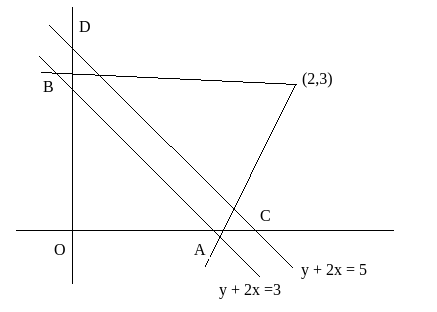
\includegraphics[width=5cm, height=3cm]{fig.png}
    
    

\end{figure}

17. Show that all chords of the curve  $2x^2-y^2-2x+4y=0$. Which subtend a right angle at the origin. Passes through a fixed point. Find the coordinates of the point.\\
18. Determine all values of a for which the point $(a, a^2)$ lies inside the triangle formed by the lines\\
$2x+3y-1=0$\\
$x+2y-1=0$\\
$5x-6y-1=0$\\
19. Tangent at a point $P_1$ [other than (0,0)] on the curve $y-x^3$ meets the curve again at $P_2$. The tangent at $P_1$ meets the curve at $P_2$ and so on . Show that the abscissae of $p_1+p_2+p_3+.....+p_n$ form a G.P. Also find the ratio.\\
20. A line through $A(5,4)$ meets the line $x+3y+2=0$ $2x+y+4=0$ and $x-y-5=0$ at points B,C and D respectively. If    $\frac{15}{AB}^2+\frac{10}{AC}^2-\frac{6}{AD}^2$, find the equation of the line.\\
21. A triangle PQRS has it's side PQ parallel to the line $y-mx$ and vertices P,Q and S on the lines $y-a$,$ x-b$ and $x--b$, respectively find the locus of the vertex R.\\
22. Using co-ordinate geometry provr that the three altitudes of any triangle are concurrent\\
23. For points $P=(x_1,Y_1)$ and $Q=(x_2,y_2)$ of the coordinate palne, a new distance $d(P,Q)$ is defined by $d(P,Q)=\mid x_1-x_2\mid + \mid y_1-y_2\mid$. Let $O=(0,0)$  and $A=(3,2)$. Prove that the set of points in the first quadrant which are equidistance (with to line new distance) from O and A consists of the union of line segment of finite length and an infinite ray. Sketch this set in a labelled diagram.\\
24. Let ABC and PQR be any two triangles in the same plane.Assume that the perpendicular from the points A,B,C to the sides QR, RP, PQ respectively are concurrent. Using vector methods or otherwise, prove that the perpendiculars from P,Q,R to BC, CA, AB  respectively are also concurrent.\\
25. Let a,b,c are real numbers with $a^2+b^2+c^2=1$. Show that the equation\\
$\Bigg |ax-by-c\hspace{1cm}bx+ay\hspace{1cm} cx+a\\
bx+ay  \hspace{1cm}ax+by-c  \hspace{1cm}cy+b\\
cx+a   \hspace{1cm} cy+b  \hspace{1cm}  ax-by+c\Bigg |$ =0\\
represents a straight line.\\
26. A straight line L through the origin meets the lines $x+y+1$ and $x+y=3$ at P and Q
respectively. Through  P and Q two straight lines $L_1 and L_2$ intersects at R . Show that the locus of R as L varies is a staight line.\\
27. A straight line negative slope passes through the points $(8,2)$ cuts the positive coordnate axes at points P and Q. Find the absolute minimum value of OP+OQ, as L varies . Where O is the origin.\\
28. The area of the triangle formed by the intersection of a line parallel to x axis and passing through $p(h,k)$ with the lines $y-x$ and $x+y-2$ is $4h^2$. Find the locus of the point .\\

\section*{H\hspace{1cm} Assertion and Reason Type Questions}


1. Lines $L_1: Y-X=0$ and $L_2 :2x+y=0$ intersects the line $l_3:y+2=0$ at P and Q, respectively. The bisector of the acute angle between $L_1 and L_2$ intersects $L_3$ at R.\\
STATEMENT-1 : The ratio $PR:RQ$equals $\sqrt[2]{2}:\sqrt{5}$. because \\
STATEMENT-2 :In any triangle, bisector of an angle divides the triangle into two triangles.\\
(a) Statement-1 is True, Statement-2 is True;Satement-2 is not a correct explaination for Statement-1\\
(b) Statement-1 is True, Statement-2 is True;Satement-2 is NOT a correct explaination for Statement-1\\
(c) Statement-1 is True, Statement-2 is False\\
(d) Statement-1 is False, Statement-2 is True\\

\section*{I\hspace{1cm} Integer Value Correct Type }

1. For a point P in the plane, let $d_1(p)$ and $d_2(p)$ bde the distance of a p point   
from the lines $x-y=0$ and $x=y=0$ respectively. The area of the region R consistes of all points P lying in the first quadrant of the plane and satisfying $2\leq d_1(p)+d_2(p)\leq$, is\\

\section*{Section-B \hspace{1cm}   JEE Main/AIEE}


1. A triangle with vertices$(4,0),(-1,-1 ),(3,5)$ is\\
(a) isoscales and right angled\\
(b) isoscales  but not right angled\\
(c) right angled but not isoscales \\
(d) neither right angled nor isoscales \\
2. Locus of mid point of the portion between the axes of $x\cos\alpha+y\sin\alpha=p$. Where p is constant is.\\
(a) $x^2+y^2=\frac{4}{p^2}$ \hspace{1cm} (b) $x^2+y^2=4p^2$\\
(c) $\frac{1}{x^2}+\frac{1}{y^2}=\frac{2}{p^2}$ \hspace{1cm}(d) $\frac{1}{x^2}+\frac{1}{y^2}=\frac{4}{p^2}$ \\
3. If the pair of lines $ax^2+2hxy+by^2+2gx+2fy+c=0$ intersects on the y-axis then\\
(a) $2fgh=bg^2+ch^2$ \hspace{1cm} (b) $bg^2\neq ch^2$\\
(c) $abc=2fgh$\hspace{1cm}  (d) none of these\\
4. The pair of lines represented by $3ax^2+5xy+(a^2-2)y^2=0$ are perpendicular to each other for \\
(a) two values of a\hspace{1cm} (b) $\forall a$\\
(c)for one value of a \hspace{1cm} (d) for no values of a\\
5. A square of side a lies above the x-axis and has one vertex at the origin. The side passing through the origin makes an angle $\alpha \left[ 0<a<\frac{\Pi}{4}]\right]$ with the positive direction of x-axis. The equation of it's diagonal passing through the origin is \\
(a) $y(\cos\alpha+\sin\alpha)+x(\cos\alpha-\sin\alpha)$=a\\
(b) $y(\cos\alpha-\sin\alpha)-x(\sin\alpha-\cos\alpha-)$=a\\
(c) $y(\cos\alpha+\sin\alpha)+x(\sin\alpha-\cos\alpha-)$=a\\
(d) $y(\cos\alpha+\sin\alpha)+x(\sin\alpha+\cos\alpha-)$=a\\
6. If the pair of straight lines $x^2-2pxy-y^2=0$ and $x^2-2qxy-y^2=0$ be such that each pair bisects the angle between the other pair, then 
(a) $pq=-1$  \hspace{1cm} (b) $p=q$  \hspace{1cm} (c) $p=-q$  \hspace{1cm} (d) $pq=1$\\
7. Locus of centroid of the triangle whose vertices are $(a\cos t, a\sin t)$, $(a\sin t,-b\cos t)$ and (1,0) where t is a parameter, is \\
(a)$(3x+1)^2+(3y)^2=a^2-b^2$\\
(b)$(3x-1)^2+(3y)^2=a^2-b^2$\\
(c)$(3x-1)^2+(3y)^2=a^2+b^2$\\
(d)$(3x+1)^2+(3y)^2=a^2+b^2$\\
8. If $x_1,x_2,x_3$ and $y_1,y_2,y_3$ are both in G.P with the same common ratio then the points $(x_1,y_1),(x_2,y_2)$ and $(x_3,y_3)$\\
(a) are vertices of a triangle\\
(b) lies on a straight line
(c) lies on elipse\\
(d) lies on circle\\
9 If the equation of the locus of a equidistance from the point $(a_1,b_1)$ and $(a_2,b_2)$ is $(a_1-b_2)x+(a_1-b_2)y+c=0$, then the value of 'c' is\\
(a) $\sqrt{a_1^2+b_1^2-a_2^2-b_2^2}$\\
(b) $\frac{1}{2}(a_2^2+b_2^2-a_1^2-b_1^2)$\\
(c) $a+1^2-a_2^2+b_1^2-b_2^2$\\
(d) $\frac{1}{2}(a_1^2+a_2^2+b_1^2+b_2^2)$\\
10. Let $A(2,-3)$ and $B(-2,3)$ be vertices of a triangle ABC. If the centroid of this triangle moves on the line $2x+3y=1$, then the locus of the vertex C is in the line \\
(a) $3x-2y=0$ \hspace{1cm} (b) $2x-3y=7$ \hspace{1cm} (c) $3x+2y=5$ \hspace{1cm} (d) $2x+=3y=9$\\
11. The equation of the straight line passing through the point (4,3) and making intercepts on the coordinate axes whose sum is -1 is \\
(a) $\frac{x}{2}-\frac{y}{3}=1$ and $\frac{x}{-2}+\frac{y}{1}=1$\\
(b) $\frac{x}{2}-\frac{y}{3}=-1$ and $\frac{x}{-2}+\frac{y}{1}=-1$\\
(c) $\frac{x}{2}+frac{y}{3}=1$ and $\frac{x}{2}+\frac{y}{1}=1$\\
(d) $\frac{x}{2}+\frac{y}{3}=1$ and $\frac{x}{-2}+\frac{y}{1}=-1$\\
12. If the sum of the slopes of the lines given by $x^2-2cxy-7y^2=0$ is four times the product c has the value\\
(a)-2 \hspace{1cm} (b)-1 \hspace{1cm} (c) 2 \hspace{1cm} (d) 1\\
13. If one of the lines given by $6x^2-xy+4cy^2=0$ is $3x+4y=0$, then c equals \\
(a) -3 \hspace{1cm} (b) -1 \hspace{1cm} (c)  3 \hspace{1cm} (d)  1\\
14. The line parallel to the x-axis and passing through the intersection of the lines $ax+2by+3b=0$ and $bx-2ay-3a=0$, where $(a,b) \neq (0,0)$\\
(a) below the x-axis at a distance of $\frac{3}{2}$ from it\\
(b) below the x-axis at a distance of $\frac{2}{3}$ from it\\
(c) above the x-axis at a distance of $\frac{3}{2}$ from it\\
(d) above the x-axis at a distance of $\frac{2}{3}$ from it\\
15. If a vertex of a triangle is (1,1) and the mid point of two sides of this vertex are (-1,2) and (3,2) then the centroid of the triangle is \\
(a) $\left[-1,\frac{7}{3}\right]$ \hspace{1cm}  (b) $\left[ \frac{-1}{3},\frac{7}{3}\right]$ \\
(c)  $\left[1,\frac{7}{3}\right]$  \hspace{1cm} (d)  $\left[ \frac{1}{3},\frac{7}{3}\right]$ \\
 16. A straigjt line through point $A(3,4)$ is such that it's intercept between the axes is bisected at A. It's equation is\\
(a)   $x+y=7$ \hspace{1cm} (b) $3x-4y+7=0$   \hspace{1cm} (c) $4x+3y=24$ \hspace{1cm}
(d) $3x+4y=25$\\
17. If $(a,a^2)$ falls inside the angle made by the lines $y= \frac{x}{2}, x>0$ and $y=3x, x>0$, then a belong to \\
(a) $\left[ 0,\frac{1}{2}\right] $ \hspace{1cm} (b) $(3,\infty)$ \hspace{1cm} (c) $\left[\frac{1}{2},3\right]$ \hspace{1cm} (d) $\left[-3,\frac{1}{2}\right]$\\
18. Let $A(h,k)$ and $B(1,1)$ and $C(2,1)$ be the vertices of a right angle triangle with AC as it's hypotenuse. If the area of the triangle is 1 square unt, then the set of values which 'k' can taken is given by\\
(a) $(-1,3)$ \hspace{1cm}(a) $(-3,-2)$\hspace{1cm} (a) $(1,3)$ \hspace{1cm}(a) $(0,2)$\\
19. Let $P=(-1,0),Q=(0,0) and R=(3,\sqrt[3]{3})$ be three points. The equation of the bisector of the angle PQR is \\
(a) $\frac{\sqrt{3}}{2}x+y=0$ \hspace{1cm} (b) $x+\sqrt{3}y=0$ \hspace{1cm} (c) $\sqrt{3}x+y=0$ \hspace{1cm}(d) $x+\frac{\sqrt{3}}{2}y=0$.\\
20. If one of the lines of $my^2+(1-m^2)xy-mx^2=0$ is a bisector of the angle between the lines $xy=0$, then m is\\
(a) 1  \hspace{1cm}(b) 2 \hspace{1cm} (c)$\frac{-1}{2}$  \hspace{1cm}(d) -2\\
21. The perpendicular bisector of the line segment joning $P(1,4)$ and $Q(k,3)$ has y-intercept -4. Then a possible value of k is\\
(a) 1 \hspace{1cm}(b) 2 \hspace{1cm}(c) -2 \hspace{1cm}(d) -4\\
22. The shortest distance between the line $y-x=1$ and the curve $x=y^2$ is \\

(a)$\frac{\sqrt{2}{3}}{8}$ \hspace{1cm} (b) $\frac{\sqrt{3}{2}}{5}$ \hspace{1cm} (c) $\frac{\sqrt{3}}{4}$ \hspace{1cm} (d) $\frac{\sqrt{3}{2}}{8}$.\\


23. The lines $p(p^2+1)x-y+q=0$ and $(p^2+1)^2x+(p^2+1)y+2q=0$ are perpendicular to a common line for \\
(a) exactly one value of p\\
(b) exactly two values of p\\
(c) more than two values of p\\
(d) no value of p\\
24. Three distinct points A,B and C are given i the 2-dimentional coordinates plane such that the ratio of the  distance of any one of them from the point (1,0) to the distance from the point (-1,0) is equal to $\frac{1}{3}$. Then the circumcenter of the triangle ABC is at the point;\\
(a) $[\frac{5}{4} ,0]$ \hspace{1cm} (b) $[\frac{5}{2} ,0]$ \hspace{1cm} (c)$[\frac{5}{3} ,0] $\hspace{1cm} (d) (0,0)\\
25. The line L given by $\frac{x}{5}+\frac{y}{b}=1$ passes through the point (13,32). The line K is parallel L and has the equation $\frac{x}{c}+\frac{y}{3}=1$. Then the distance between L and K is \\
(a)$\sqrt{17}$  \hspace{1cm} (b)$\frac{17}{\sqrt{15}}$ \hspace{1cm} (c)$\frac{23}{\sqrt{17}}$ \hspace{1cm} (d) $\frac{23}{\sqrt{15}}$\\
 26.The line $L_1:y-x=0$ and $L_2: 2x+=y=0$ intersects the line $L_3: y+2=0$ at P and Q respectively. The bisector of the acute angle between $L_1 and L_2$ intersects $L_3$ at R\\
 STATEMENT-1: The ratio PR;RQ equals $\sqrt[2]{2}:\sqrt{5}$\\
 STATEMENT-2: In any triangle,bisector of an angle divides the triangle into two similar triangles.\\
(a) Statement-1 is True, Statement-2 is True,Statement-2 is not a correct explaination for the Statement-1.\\
(b) Statement-1 is True, Statement-2 is False\\
(c) Statement-1 is False, Statement-2 is True\\
(d) Statement-1 is True, Statement-2 is True,tatement-2 is correct explaination for the Statement-1.\\
27. If the line $2x +y=k$ passes through the point which divides the line segment joining the points $(1,1)$ and (2,4) in the ratio $3:2$,then k equals:\\
(a) $\frac{29}{5}$ \hspace{1cm} (b) 5 \hspace{1cm} (c) 6 \hspace{1cm} (d) $\frac{11}{5}$\\
28. A ray of light along $x+\sqrt{3}y=\sqrt{3}$ get reflected upon reaching x-axis,the equation of the reflected ray is\\
(a)$y=x+\sqrt{3}$ \hspace{1cm} (b) $\sqrt{3}y=x-\sqrt{3}$ \hspace{1cm} (c)$y=\sqrt{3}x-\sqrt{3}$ \hspace{1cm} (d) $\sqrt{3}y=x-1$ \\
29. The coordinate of the incenter of the triangle that has the coordinates of mid points of it's sides as (0,1) (1,1) and (1,0) is;\\
(a) $2+\sqrt{2}$\hspace{1cm} (b) $2-\sqrt{2}$ \hspace{1cm} (c) $1
+\sqrt{2}$ \hspace{1cm} (d) $1-\sqrt{2}$\\
30. Let PS e the median of the triangle with vertices $P(2,2)$,$Q(6,-1)$ and $R(7,3)$. The equation of the line passing through (1,-1)and parallel to PS is:\\
(a) $4x+7y+3=0$ \hspace{1cm} (b) $2x-9y+11=0$ \hspace{1cm} (c)
$4x-7y+11=0$ \hspace{1cm} (d) $2x+7y+9=0$ \\
31. Let a,b,c and d be non-zero numbers. If the point of intersection of the lines $4ax+2ay+c=0$ and $5bx+2by+d=0$ lies in the fourth quadrant and eqidistance from the two axes then \\
(a) $3bc_2ad=0$  \hspace{1cm} (b) $3bc+2ad=0$\hspace{1cm} (c) $2b-3ad=0$ \hspace{1cm} (d) $2bc+3ad=0$\\
32. The number of points, having both co-ordinates as integers, that lie in the interior of the triangle ith vertices (0,0)(0,41) and(41,0)is.\\
(a) 820 \hspace{1cm} (b) 780 \hspace{1cm} (c)901 \hspace{1cm} (d) 861\\
33. Two sides  of a rhombus are alon the lines, $x-y+1=0$ and $7x+y-5=0$. If it's diagoals intersect at(-1,-2), then which one of the following is a vertex of this rhombus?\\
(a) $\left[ \frac{1}{3},\frac{8}{3}\right]$ \hspace{1cm} (b) $\left[ \frac{10}{3},\frac{7}{3}\right]$ \hspace{1cm} (c)$(-3,-9)$ \hspace{1cm} (d) $(-3,-8)$\\
34. A straight the thrugh a fixed point (2,3)intersects the coordinate axes at distinct point P  and Q. If O is the origin and the rectangle OQPR is completed, then the locus of R is:\\
(a) $2x+3y=xy$ \hspace{1cm} (b) $3x+2y=xy$ (c) $3x+2y=6xy$ \hspace{1cm} (d) $3x+2y=6$\\
35.Consider the set of all lines $px+qy+r=0$ such that $3p+2q+4r=0$. Which one of the following statements is true?\\
(a) The lines are concurent at the point $\left[ \frac{3}{4}\frac{1}{2}\right] $.\\
(b) Each the line passes through the origin.\\
(c) The lines are parallel.
(d) The lines are not concurrent.\\
36. Slope of line passing through $P(2,3)$ and intersecting the line $x+y=7$ at a distance of 4units from  P,  is :\\
(a)$\frac{1-\sqrt{5}}{1+\sqrt{5}}$\hspace{1cm} (b) $\frac{1-\sqrt{7}}{1+\sqrt{7}}$\hspace{1cm} (c) $\frac{\sqrt{7}-1}{\sqrt{7}+1}$\hspace{1cm} (d)$\frac{\sqrt{5}-1}{\sqrt{5}+1}$\\
 \end{document}   